\section{项目内容}

\subsection{整体架构}

\subsubsection{系统整体架构}
系统的主要由以下部分构成:
\begin{enumerate}
    \item 运行于主计算机ROS(机器人操作系统)上的算法与决策层
    \item 运行于Xilinx ZYNQ 7020芯片上的ROS系统的上的硬件接口层, 用于对主计算机难以直接控制的硬件进行信号采集和驱动
    \item 深度摄像头Kinect, 用于初步的物体识别
    \item 机械臂, 用于物体抓取
    \item 机械臂末端摄像头与超声波传感器,用于末端的目标位置修正与反馈
    \item 机器人移动平台,用于扩展机械臂的抓取范围
\end{enumerate}

各个部分之间的连接方式如图\ref{fig:structure}所示。\ 
\begin{figure}[ht]
    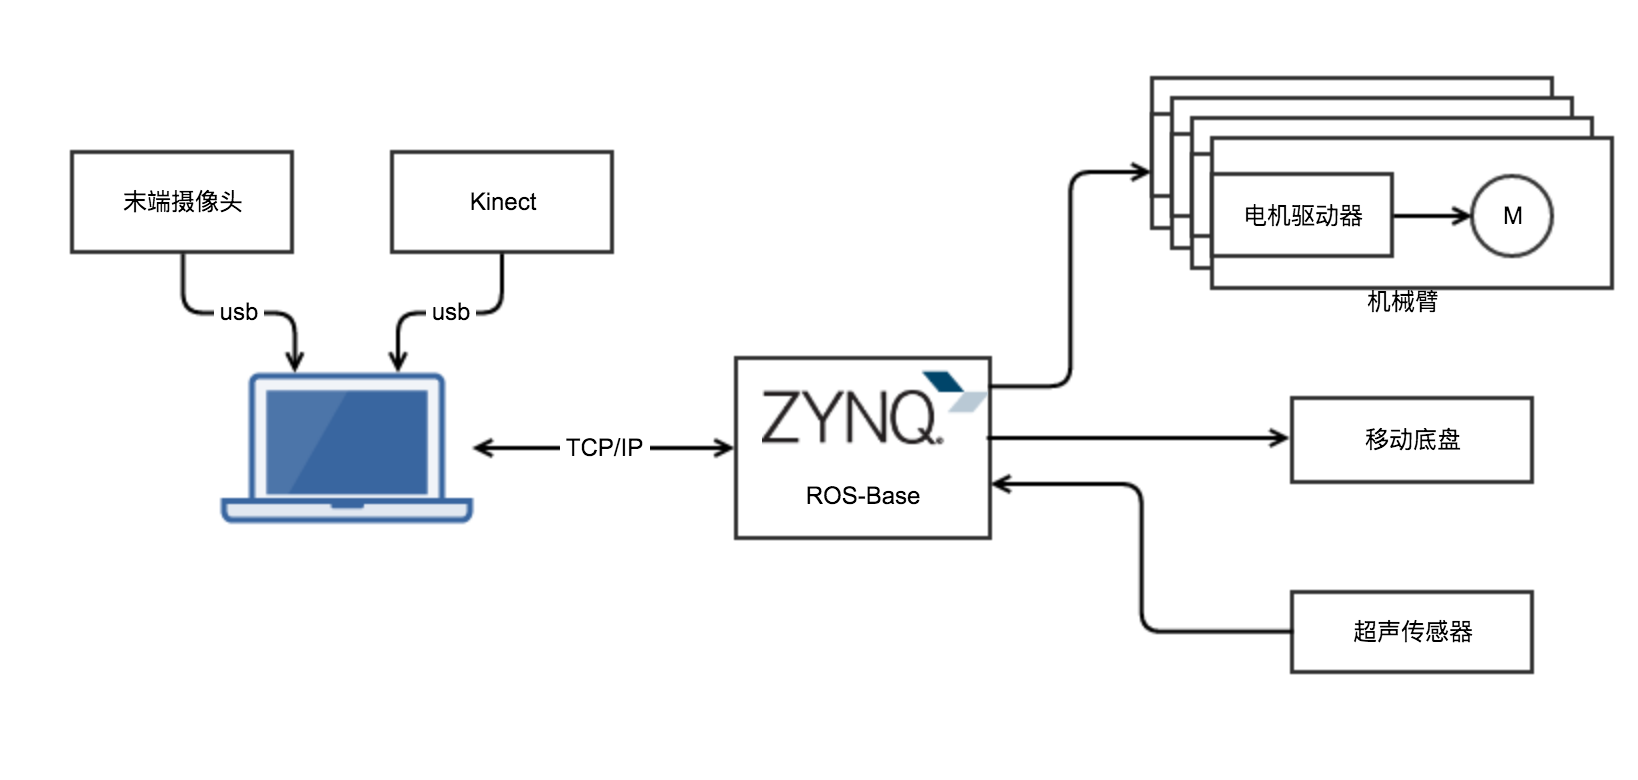
\includegraphics[width = \textwidth]{images/arch.png}
    \caption{整体系统架构}
    \label{fig:structure}
\end{figure}

\subsubsection{通信架构设计思路}
系统整体的硬件通信架构基于机器人操作系统ROS构建。\ ROS是一个基于网络协议的通信系统,支持分布式的节点。\ 
在主机器人上运行的节点负责图像处理与机械臂的运动规划。\ 规划的结果通过网络发送到同样运行着ROS的ZYNQ芯片上。\ 
ZYNQ芯片是一种同时集成了ARM微处理器和FPGA可编程逻辑的全可编程器件。\ 在FPGA上构建了用于直接控制电机并且采集超声波传感器反馈的外设。\ 
而在微处理器上运行的ROS节点通过网络从主计算机运行的ROS节点上收到控制机械臂姿态目标,转换为实际电机的PWM脉宽写入电机控制外设。\ 
同时另一个ROS节点采集超声反馈信息通过网络发送到主计算机上用于之后的运动规划。\ 

\subsubsection{视觉系统设计思路}
Kinect深度摄像头可以给出0.6m到4.5m之内的立体图像。\ 通过图像处理方法分辨出深度图像中的物体。\ 然而由于Kinect深度摄像头本身的分辨率和净度所限,会产生深度和位置信息不准确以及误报物体等情况。\ 

为了修正这些误差,我们使用了一个机械臂末端的摄像头。\ 主计算机从末端摄像头图像中提取出可能的物体区域,和预先采集的物品图像库进行匹配。\ 如果匹配失败,就认为该物品为Kinect误报。\ 如果匹配成功就开始物品的抓取,在抓取过程中利用末端摄像头看到的物品图像进行反馈。\ 反馈目标为将物品图像定位到末端摄像头图像的中心,同时通过超声波传感器信息采集机械手到物体的距离就可以达到准确抓取的效果。\ 

实际抓取过程的详细流程图如图\ref{fig:flowchart}所示。\ 

\begin{figure}
	\centering
    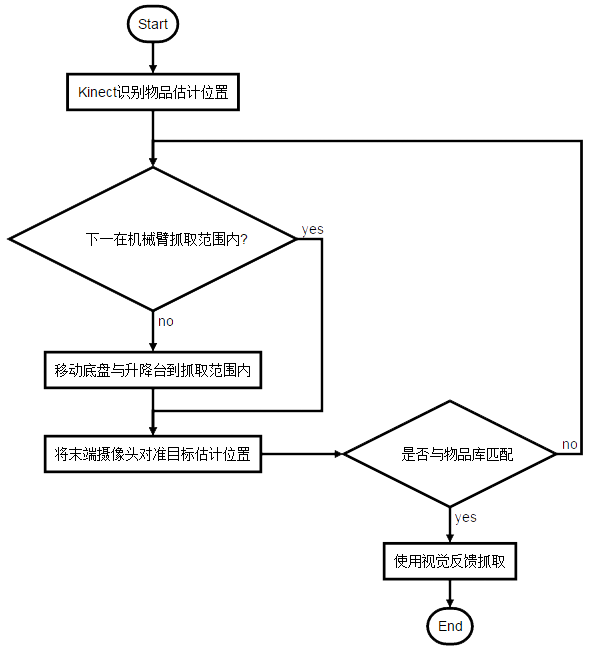
\includegraphics[width = 0.9\textwidth]{images/flow.png}
    \caption{抓取流程图}
    \label{fig:flowchart}
\end{figure}

\subsubsection{坐标定义}

在整个抓取过程中使用的坐标定义如下:
\begin{enumerate}
    \item 机器人本体坐标系 base\_link, 以机器人正前方为x轴,正左方为y轴的右手系
    \item Kinect坐标系 kinect\_link,以kinect正左方为x轴,正上方为y轴的右手系
    \item 末端视觉坐标系 hand\_link,以机械手正前方为x轴,正左方为y轴的右手系
\end{enumerate}

\subsection{项目设计及实现细节}
\subsubsection{图像处理}
\paragraph{灰度熵}

以图\ref{fig:registered}为例,我们将演示分离书架上的物体和书架的算法。\ 直接利用灰度熵,去除书架背景,结果如图\ref{fig:entropy_block}所示。\ 对于一张给定的图片,其熵的定义如下:
\begin{equation}
	E = -\Sigma p_{i} \cdot \log_{2}p_{i}
\end{equation}

\begin{figure}[H]
\begin{minipage}[t]{0.5\textwidth}
	\centering
    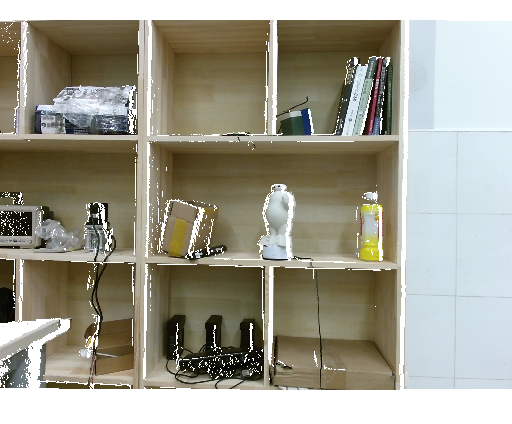
\includegraphics[width = 0.8\textwidth]{images/registered.png}
    \caption{示例图片}
    \label{fig:registered}
\end{minipage}
\begin{minipage}[t]{0.5\textwidth}
	\centering
    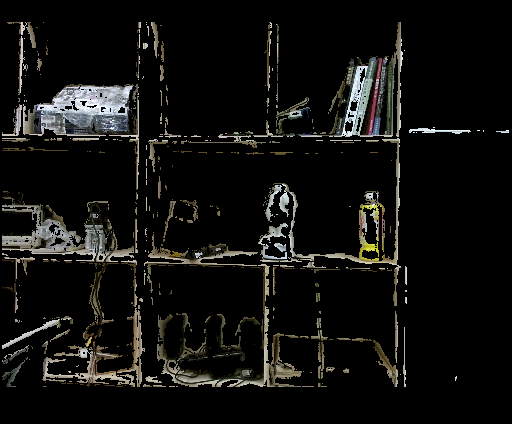
\includegraphics[width = 0.8\textwidth]{images/entropy_block.png}
    \caption{灰度熵结果}
    \label{fig:entropy_block}
\end{minipage}
\end{figure}

在这张图片中,书架被过滤得很干净。\ 不过那些纯色的物体也被过滤了。\ 此外,书架的框架也没有去除干净,所以这张图片还不能用于目标的定位和识别。\ 针对熵过滤的不足,我们又提出了色块检测、线段检测方法。\     
    
\paragraph{色块检测}

在图片进行边缘检测之后,降采样,找到其中的纯色块。\ 其中位于边缘部分的色块意义不大,直接忽略,结果如图\ref{fig:downsampled_filled}。\ 

\begin{figure}[H]
\begin{minipage}[t]{0.5\textwidth}
	\centering
    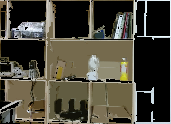
\includegraphics[width = 0.8\textwidth]{images/downsampled_filled.png}
    \caption{色块检测结果}
    \label{fig:downsampled_filled}
\end{minipage}
\begin{minipage}[t]{0.5\textwidth}
	\centering
    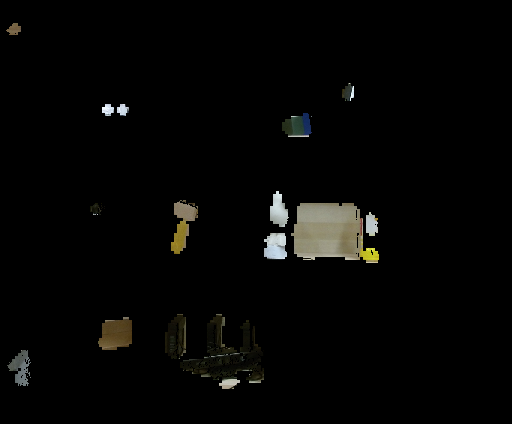
\includegraphics[width = 0.8\textwidth]{images/color_block.png}
    \caption{色块分离结果}
    \label{fig:color_block}
\end{minipage}
\end{figure}

这些色块中,既有背景色块,又有目标色块,需要将他们分离。\ 首先,将剩余色块中面积最大的色块视为标准背景色块(如果标准背景色块的面积比较小,则认为所有色块均为目标色块,终止背景色块识别操作)。\ 检查所有色块,面积同标准背景色块相近、或者颜色同标准背景色块类似的色块,均被视为背景色块。\ 其余的部分直接视作目标色块。\ 最后,将降采样的结果重新应用到图片上,获得图片的色块层,如图\ref{fig:color_block}。\ 

可以观察到色块检测也存在缺陷,在背景颜色起伏较大的细节区域可能无法准确辨别背景色块和目标色块。\ 这些区域将会在平面检测时过滤。\ 

\paragraph{线段检测}

在图片进行边缘检测之后,降采样,如图\ref{fig:raw_contour}所示。\ 将边缘点过分密集的区域清理掉,这些特征点密集的区域应当是目标,结果如图\ref{fig:after_contour}。\ 	
\begin{figure}[H]
\begin{minipage}[t]{0.5\textwidth}
	\centering
    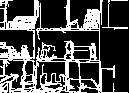
\includegraphics[width = 0.8\textwidth]{images/raw_contour.png}
    \caption{边缘检测结果}
    \label{fig:raw_contour}
\end{minipage}
\begin{minipage}[t]{0.5\textwidth}
	\centering
    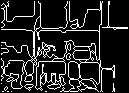
\includegraphics[width = 0.8\textwidth]{images/after_contour.png}
    \caption{边缘区域清理结果}
    \label{fig:after_contour}
\end{minipage}
\end{figure}

实践时发现,纯色块的边缘也可能被意外地检测为线段,所以将纯色块区域附近的边缘删除,如图\ref{fig:final_contour}。\ 最后,使用Hough检测其中的线段,结果如图\ref{fig:lines}。\ 

\begin{figure}[H]
\begin{minipage}[t]{0.5\textwidth}
	\centering
    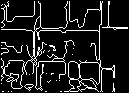
\includegraphics[width = 0.8\textwidth]{images/final_contour.png}
    \caption{纯色快边缘删除结果}
    \label{fig:final_contour}
\end{minipage}
\begin{minipage}[t]{0.5\textwidth}
	\centering
    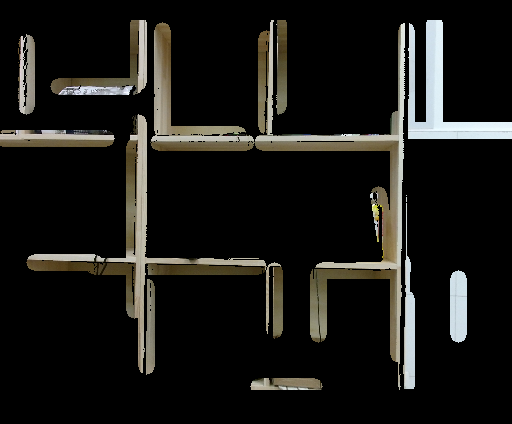
\includegraphics[width = 0.7\textwidth]{images/lines.png}
    \caption{线段检测结果}
    \label{fig:lines}
\end{minipage}
\end{figure}
    
\paragraph{总结}

最后,我们可以合成得到目标图层:

\begin{figure}[H]
	\centering
    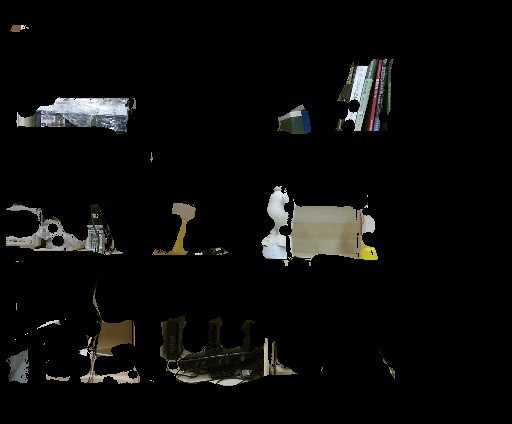
\includegraphics[width = 0.4\textwidth]{images/object.png}
    \caption{最终结果}
    \label{fig:object}
\end{figure}

\subsubsection{深度视觉}

利用Kinect2我们可以获取场景的RGB图像,以及RGB图像中每一个点对应的到镜头的距离。\ 我们完成对Kinect2设备的标定后,就获得了深度信息到机器人坐标的变换矩阵,这样每一个对应的二维图层都可以转化为与之对应的三维点云模型。\ 

\begin{figure}[H]
\begin{minipage}[t]{0.5\textwidth}
	\centering
    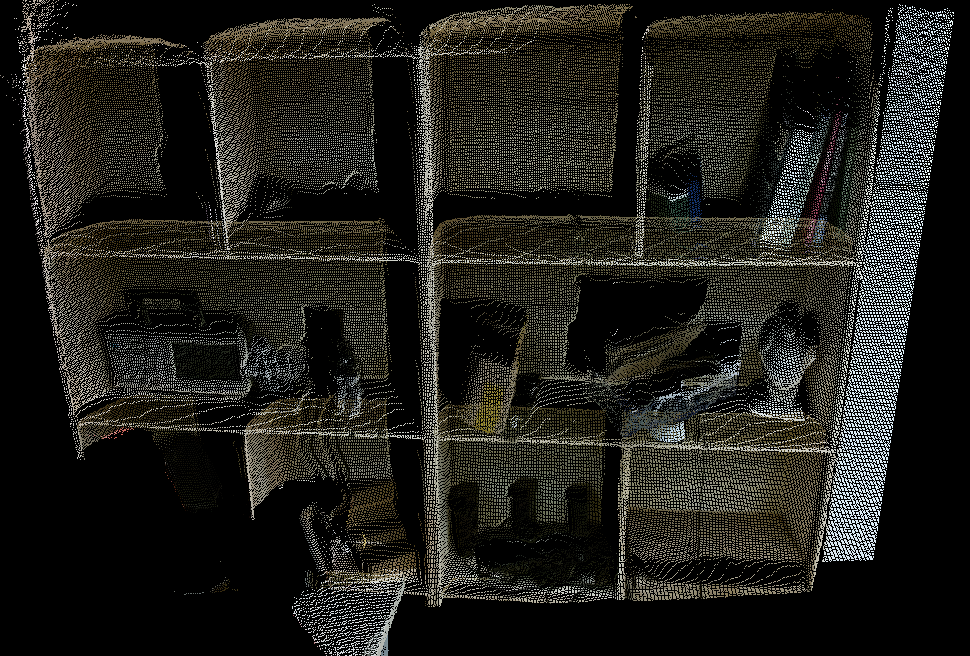
\includegraphics[width = 0.8\textwidth]{images/00.png}
    \caption{原始点云}
    \label{fig:initial_pc}
\end{minipage}
\begin{minipage}[t]{0.5\textwidth}
	\centering
    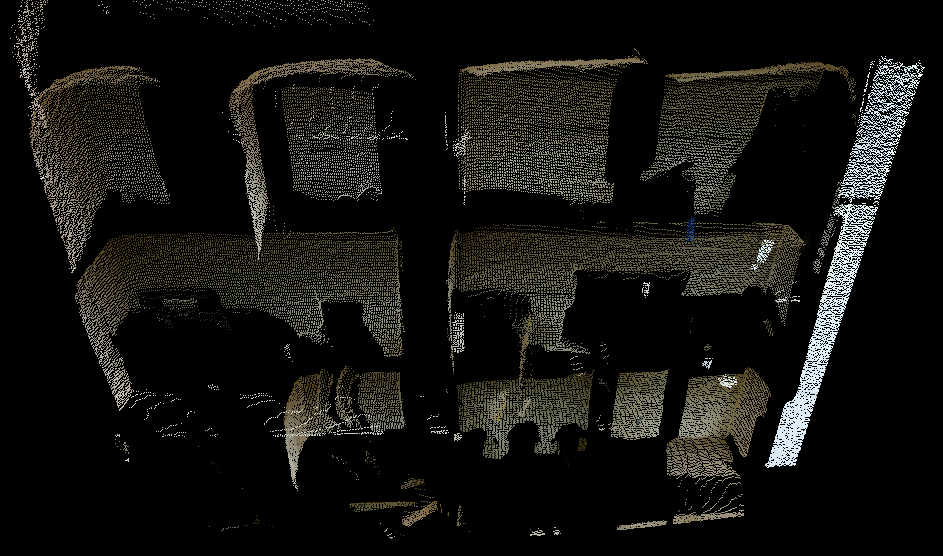
\includegraphics[width = 0.9\textwidth]{images/01.png}
    \caption{确定的背景}
    \label{fig:bg}
\end{minipage}
\end{figure}

为了进一步清理RGB过滤中获取的信息,实现目标的准确定位,我们将利用目标图层和书架背景图层对应的三维模型进行深度信息的处理。\ 我们在书架背景图层中找到一个最大的平面作为墙面,以墙面的坐标为基准,去除目标图层中在那些在墙面上的点。\ 最后,我们对清理后的背景图层进行欧几里得聚类,将每一组几何关系上相互连接的点认作是一个目标,完成全部目标的定位工作。\ 

\begin{figure}[H]
\begin{minipage}[t]{0.5\textwidth}
	\centering
    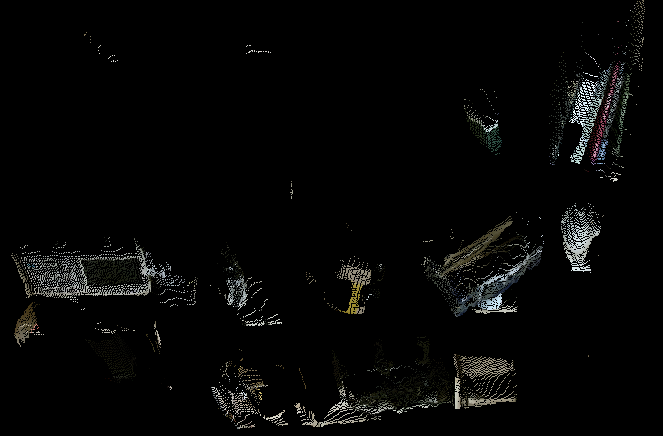
\includegraphics[width = 0.85\textwidth]{images/02.png}
    \caption{物体图层}
    \label{fig:obj}
\end{minipage}
\begin{minipage}[t]{0.5\textwidth}
	\centering
    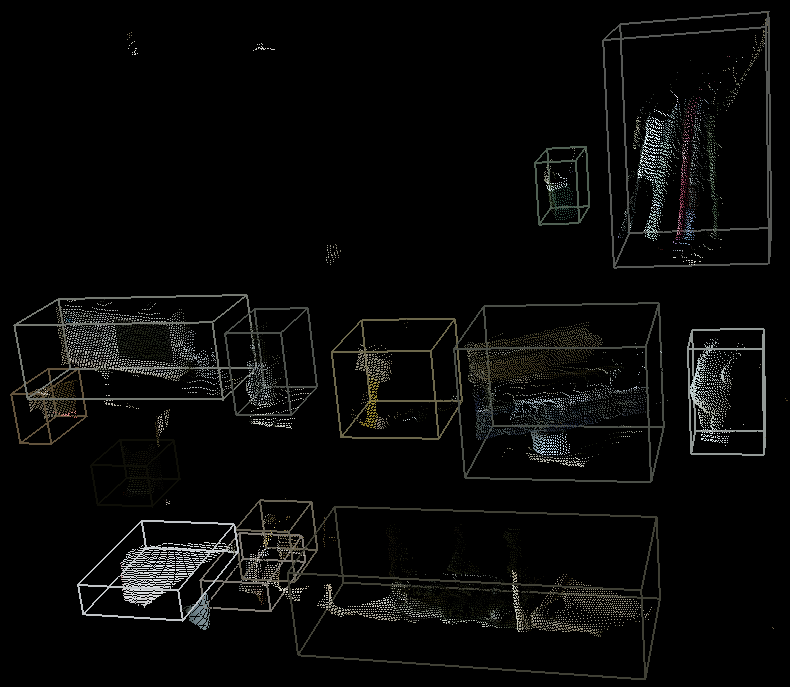
\includegraphics[width = 0.65\textwidth]{images/03.png}
    \caption{聚类后的物体图层}
    \label{fig:clustering}
\end{minipage}
\end{figure}

\begin{figure}[H]
\begin{minipage}[t]{0.5\textwidth}
	\centering
    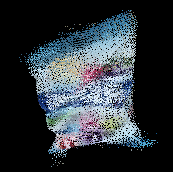
\includegraphics[width = 0.7\textwidth]{images/04alp.png}
    \caption{糖果袋}
    \label{fig:alp}
\end{minipage}
\begin{minipage}[t]{0.5\textwidth}
	\centering
    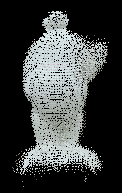
\includegraphics[width = 0.45\textwidth]{images/05baymax.png}
    \caption{Baymax模型}
    \label{fig:baymax}
\end{minipage}
\caption{物体点云}
\end{figure}

\subsubsection{末端视觉}

我们从末端摄像头获得原始图像,其分辨率为$640\times480$,以$10$Hz的频率从摄像头读取,并且包装成ros信息后被发布,供后续模块读取。\ 正如上一部分所说,对于室内场景的图片,我们可以使用灰度熵来处理图像,对于末端视觉我们也采用了这种方法。\ 处理之后我们便获得了物体的图像,接着我们需要辨别物体的类型。\ 作为前提,我们不妨直接取所有物体中轮廓最大的那个作为研究的目标物体。\ 

\paragraph{物体识别}

我们使用 基于稀疏表示的分类器(Sparse Representation-based Classification)对上述的图像进行识别。\ 首先,我们事先准备该物体一定数量的样本,并假设当样本数量足够时,每张该物体的照片都可以近似表示为该物体样本照片的线性叠加,并且与其他物体的样本照片线性无关,这也就是“稀疏表示”的含义。\ 数学形式的表示为:
\begin{equation}
\boldsymbol{y} = A\,\boldsymbol{x_{0}} 
\end{equation}
其中$\boldsymbol{x_{0}} = [0, ..., 0, a_{i, 1}, ..., a_{i, n_{i}}, 0, ..., 0]$,若该物体属于第$i$类。\ 

可以证明\cite{wright2009robust},稀疏解$x_{0}$可以近似的被如下的表达式所估算:
\begin{equation}
\label{stable_l1}
\hat{x_{1}} = \text{arg}\ \text{min} ||\boldsymbol{x} ||_{1} \qquad\text{s.t.}\: ||A\boldsymbol{x}-\boldsymbol{y}||_{2} \leq \varepsilon 
\end{equation}

并且可以证明,$\hat{x_{1}}$能充分接近$\hat{x_{0}}$。\ 具体的实现方法如下:

\begin{enumerate}
\item 首先给定一系列样本矩阵$\mathbf{A}$,被测试样例$\boldsymbol{y}$,以及可容忍误差$\varepsilon$;
\item 将$\mathbf{A}$标准化使其有单位的$L_2$范数,然后求解方程\eqref{stable_l1};
\item 依次计算残差$r_{i}(\boldsymbol{y}) = ||\boldsymbol{y}-A\delta_{i}(\hat{x_{1}})||_{2}$,其最小值即为我们识别的结果。\ 
\end{enumerate}

\paragraph{降采样}

为了降低$\boldsymbol{y}$的维数,从而加快运算速度,对图片进行特征提取是很有必要的。\ 从数学上可以证明,只要提取的特征向量的维度大于$O( \log n)$,就不会影响方程\eqref{stable_l1}的解,因此我们可以直接对图片进行降采样。\ 

\subsubsection{机械臂设计}

\paragraph{结构设计思路}

选用的舵机能够负载$30$N$\cdot$m,舵机行程共$270^\circ$左右,动力充足,行程宽,故希望能够将舵机的有效行程缩短至所需的范围,以此优化机械臂的动力分配性能。

\paragraph{第一版}

如图\ref{fig:arm1}所示,第一版机械臂为兼容延续之前的机械设计以及成果,采用了较为灵活的钣金结构设计,沿用了前作的底座,有效的节省了设计周期与成本。

\begin{figure}[H]
    \centering
    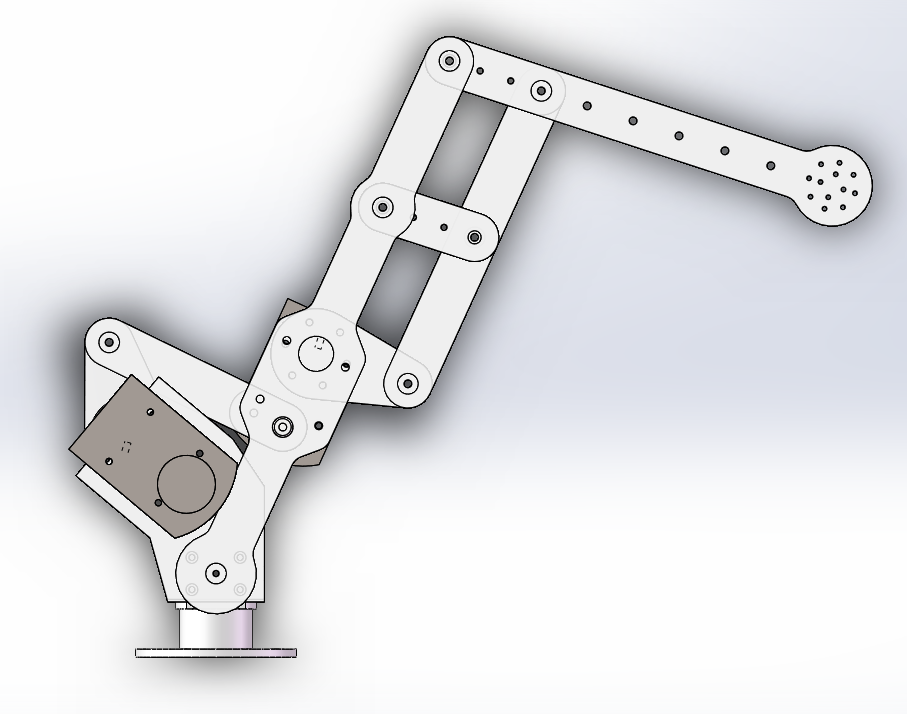
\includegraphics[width = 0.75\textwidth]{images/arm_1.png}
    \caption{第一版机械臂外观}
    \label{fig:arm1}
\end{figure}

在图\ref{fig:arm2}中可以看到有关机械臂的设计的原始尺寸,其主要目的为规划舵机的行程,使得行程充分转化,以达到优化的目的。

\begin{figure}[ht]
\begin{minipage}[t]{0.5\textwidth}
    \centering
    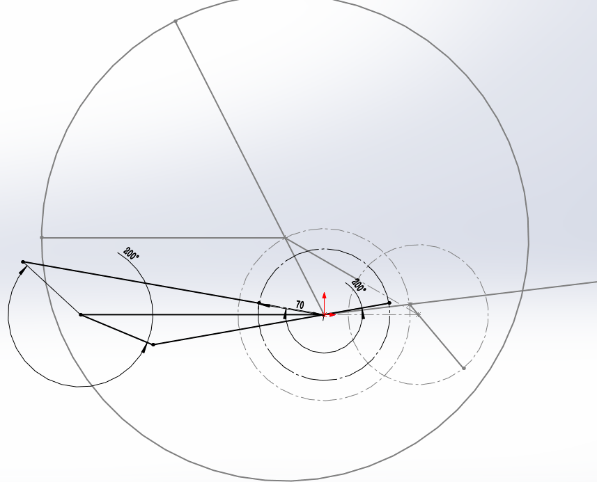
\includegraphics[width = 0.9\textwidth]{images/arm_2.png}
\end{minipage}
\begin{minipage}[t]{0.5\textwidth}
    \centering
    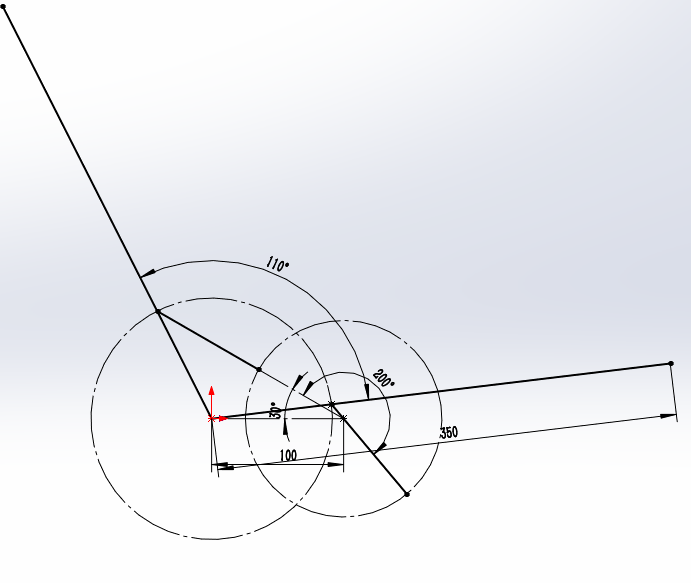
\includegraphics[width = 0.9\textwidth]{images/arm_3.png}
\end{minipage}
\caption{机械臂行程规划图}
\label{fig:arm2}
\end{figure}

如图\ref{fig:arm4}所示,第一版机械臂的载荷(蓝色)随机械臂上提而减小,同时机械臂的动力却在逐渐上升,从而在运动的中后段能够灵活有效的运动,但在前段会出现一段较大的动力不足的区间。

\begin{figure}[H]
    \centering
    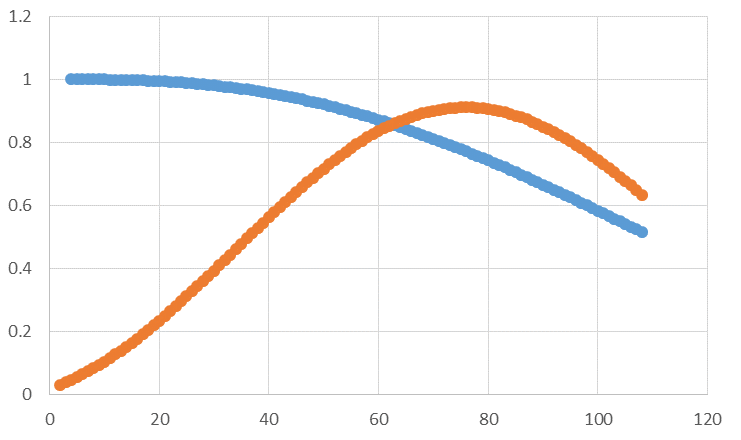
\includegraphics[width = 0.75\textwidth]{images/arm_4.png}
    \caption{第一版机械臂负载与载荷关系}
    \label{fig:arm4}
\end{figure}

第二版:如图\ref{fig:arm5}所示,第二版在前一版的基础之上加装了一个自由度,同时增加了许多的横向加固的内梁结构,能够有效的解决前一版机械臂抗扭曲刚度不足的问题。

\begin{figure}[H]
    \centering
    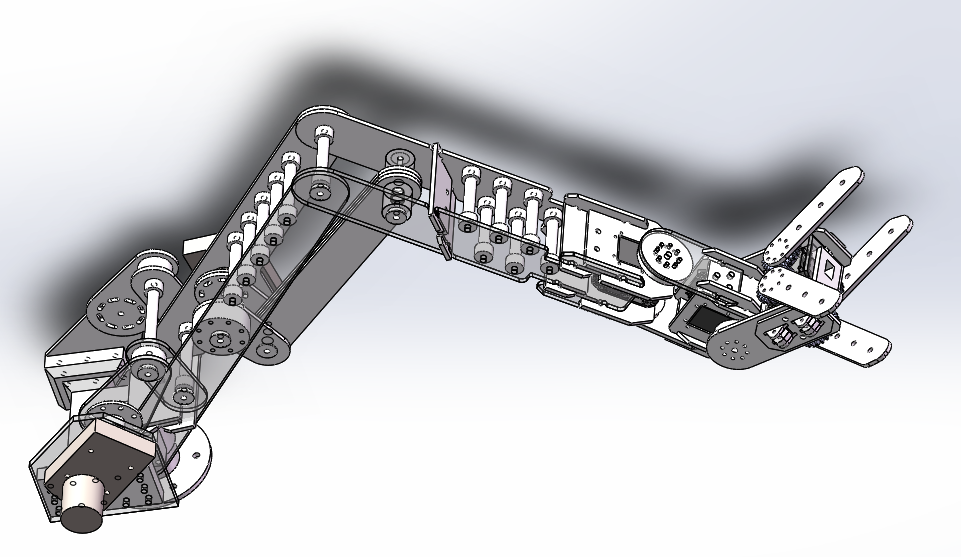
\includegraphics[width = 0.75\textwidth]{images/arm_5.png}
    \caption{第二版机械臂总成图}
    \label{fig:arm5}
\end{figure}

如图\ref{fig:arm6}所示,在第二版的机械臂设计中,吸取了上一版的机械臂的长处与优点,并且针对前一半的机械臂在前半段的运动区间内有较大的动力不足的情况作出了改进,改进后的载荷与负载关系如图\ref{fig:arm7}所示。

\begin{figure}[ht]
\begin{minipage}[t]{0.35\textwidth}
    \centering
    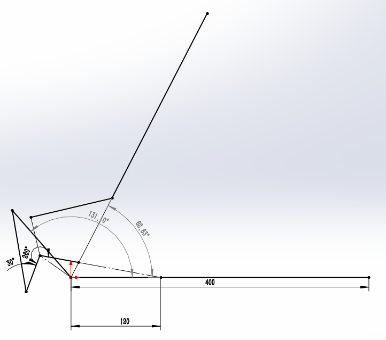
\includegraphics[width = 0.9\textwidth]{images/arm_6.png}
\end{minipage}
\begin{minipage}[t]{0.65\textwidth}
    \centering
    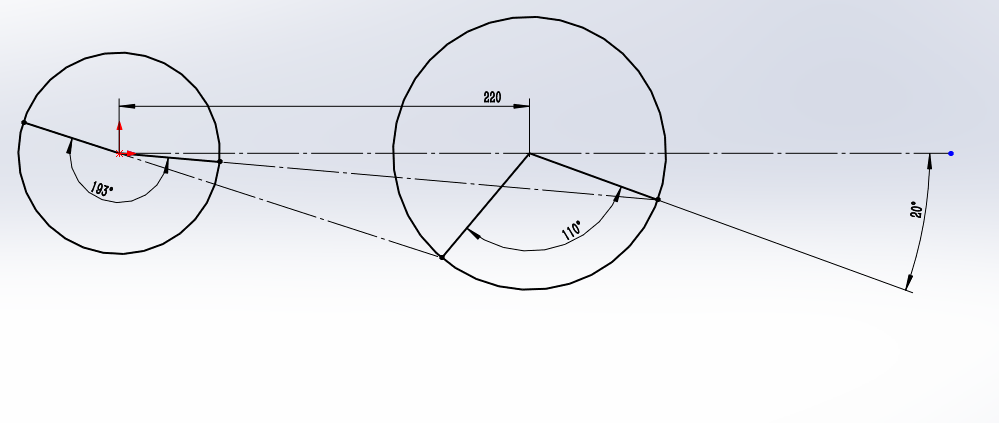
\includegraphics[width = 0.9\textwidth]{images/arm_7.png}
\end{minipage}
\caption{机械臂行程规划图}
\label{fig:arm6}
\end{figure}

\begin{figure}[H]
    \centering
    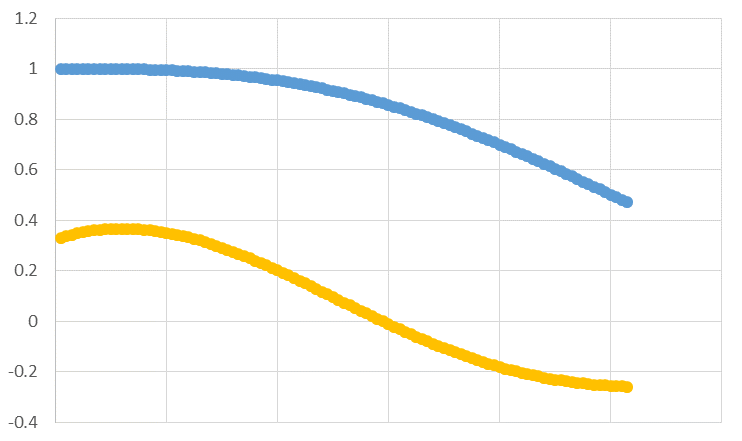
\includegraphics[width = 0.75\textwidth]{images/arm_8.png}
    \caption{第二版机械臂动力分配效果}
    \label{fig:arm7}
\end{figure}

\paragraph{其他创新设计}

在第二版的机械臂设计中,拟增加自适应机械手环节,使得$70$N$\cdot$m的舵机能够发挥充足的握力,拥有臂上一版更加优良的抓持稳定性,其自适应手结构目前仍在设计阶段,初期尺寸规划及行程安排如图\ref{fig:arm8}。

\begin{figure}[H]
    \centering
    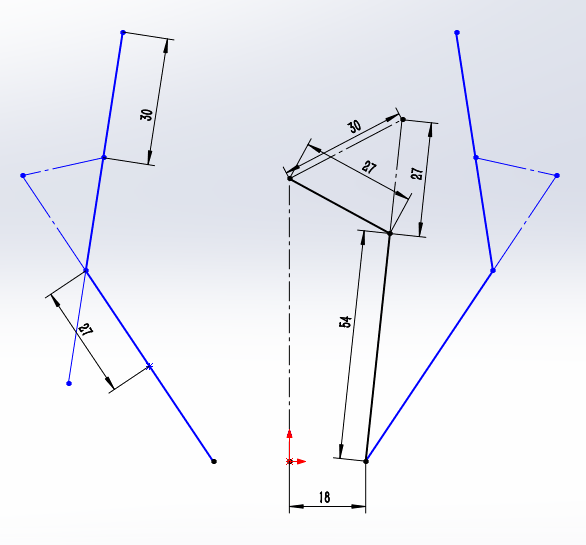
\includegraphics[width = 0.6\textwidth]{images/arm_9.png}
    \caption{自适应手关节初期设计草图}
    \label{fig:arm8}
\end{figure}

\subsubsection{机械臂控制}

考虑到控制算法的可扩展性,我们采用了通用的机械臂位姿算法。\ 首先,建立机械臂对象,输入机械臂每一段的转轴方向、相对于下一个关节的位移即可。\ 在建立了模型后,便可通过机械手的目标位置解算出电机的目标角度。\ 求解时采用了一种非线性优化算法,LM算法(Levenberg-Marquardt)\cite{more1978levenberg}。\ 它将高斯-牛顿法与梯度下降法相结合,从初始点开始迭代,通过合适的阻尼因子$\lambda$来达到最终解。\ 这个算法能够有效处理冗余参数的问题,在处理实际问题时效果良好。\ 

在具体的实现过程中,由于算法对初值敏感,所以我们会在机械臂当前角度作为初值求解失败后采用随机的角度作为初值重复求解直至得到结果。\ 

在每一次抓取物体之前,机械臂会回到初始位置,从深度视觉获得目标物体的三维位置信息作为机械手的初始目标。\ 机械手向前移动,在此过程中不断接收末端摄像头识别出的物体位置,依此在yz平面上调整目标位置,形成闭环控制。\ 距离传感器不断探测机械手与物体的距离,在到达阈值后让机械手上的电机转动,抓取物体。\ 

\begin{figure}[H]
    \centering
    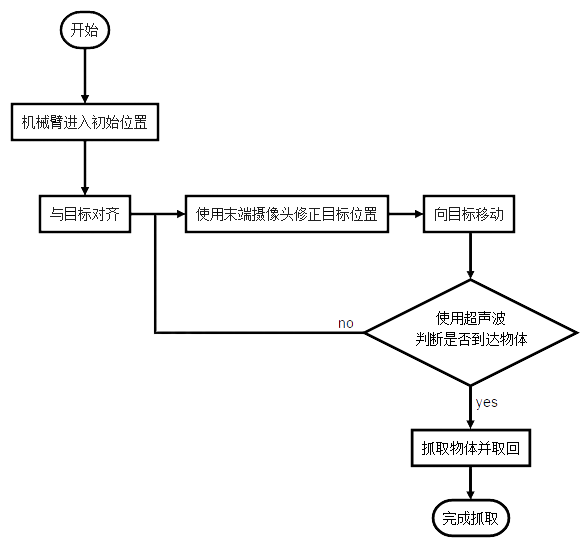
\includegraphics[width = 0.8\textwidth]{images/arm.png}
    \caption{机械臂流程图}
    \label{fig:arm}
\end{figure}

另外,为了保证深度视觉信息的准确,在Kinect2获取场景图像前,机械臂将旋转至一个边缘位置,到Kinect2的视野之外,减小对于图像与深度信息的干扰。\ 

\subsubsection{距离传感器}

由于单目的末端摄像头无法准确获得物体的深度信息,通过深度视觉获取的深度信息精度也无法保证,所以我们在机械手上加装了末端超声波传感器,用来准确探测与目标物体之间的距离。\ 在距离达到阈值后,便告知机械臂已到达目标位置,可以开始抓取物体。\ 

\subsubsection{移动底盘}

在底盘设计中,原本采用四个独立正交的欧姆尼轮作为运动输出,但在实际使用过程中发现该设计的通过性较弱,不能够适应复杂的环境,容易被线缆等物体牵制。故在后续的设计中,我们采用麦克纳姆轮作为动力输出,使得底盘能够在保持全向运动性的同时获得更大的带载能力与更好的通过性。

\begin{figure}[ht]
\begin{minipage}[t]{0.35\textwidth}
    \centering
    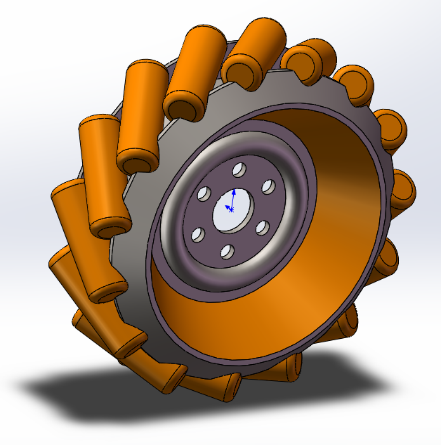
\includegraphics[width = 0.9\textwidth]{images/chassis_1.png}
\end{minipage}
\begin{minipage}[t]{0.65\textwidth}
    \centering
    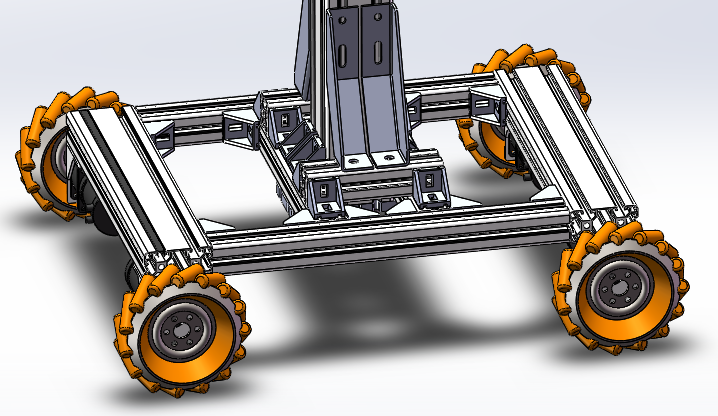
\includegraphics[width = 0.9\textwidth]{images/chassis_2.png}
\end{minipage}
\caption{麦克纳姆轮及底盘}
\label{fig:cha1}
\end{figure}

同时,在新的底盘设计设计中,采用了6063铝型材作为底盘的主框架,有效的增加了底盘的可扩展性与比强度,简化了设计的难度。

\begin{figure}[H]
    \centering
    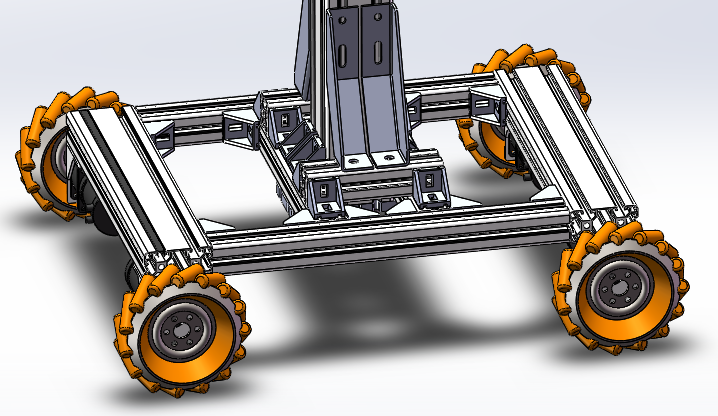
\includegraphics[width = 0.6\textwidth]{images/chassis_2.png}
    \caption{选用的欧标6063铝型材横截面示意图}
    \label{fig:cha2}
\end{figure}
